\section{Đường đi bao phủ} 
Ngày nay, khi nhiệt độ trái đất nóng lên từng ngày các thảm hoạ thiên nhiên cháy rừng đang ngày một xuất hiện nhiều hơn với mức độ nghiêm trọng. Việc biêt càng sớm về thảm hoạ con người càng có lợi thế để giảm thiểu thiệt hại cũng như khống chế đám cháy. Tuy nhiên với một diện tích lớn bất kỳ chúng ta có các giới hạn về mặt triển khai thiết bị. Để khắc phục vấnđề đấy việc sử dụng các máy bay không người lái là lựa chọn tối ưu. Một vấn đề liên quan là hoạch định đường đi cho xe để khi đường đi theo toàn bộ địa hình (khu vực mục tiêu) được quét. Vấn đề như vậy được gọi là lập kế hoạch lộ trình bao phủ. Bài viết trình bày một chiến lược tập trung vào việc xây dựng một bầy Robot hình thành đội hình chữ V và tạo ra một tuyến đường đặc biệt tối ưu phục vụ cho hoạt động tuần tra và giám sát một vùng lồi quan tâm

Coi khu vực khảo sát là một đa giác lồi. Đàn Robot cất cánh và hạ cánh lần lượt tại điểm đầu $P_s$ và điểm cuối $P_e$, như minh họa trong Hình.\Ref{fig:SW1}. Trong phần này, chiến lược đi tiến lùi được thực hiện để tạo ra một đường bao phủ tối ưu trong đó bầy đàn theo dõi các đường thẳng, được gọi là đường đi, bên trong khu vực khảo sát và chiến lược bao phủ quét của đội hình Robot hình chữ V sử dụng phạm vi bao phủ được thiết kế.

    \begin{figure}[h]
        \centering
        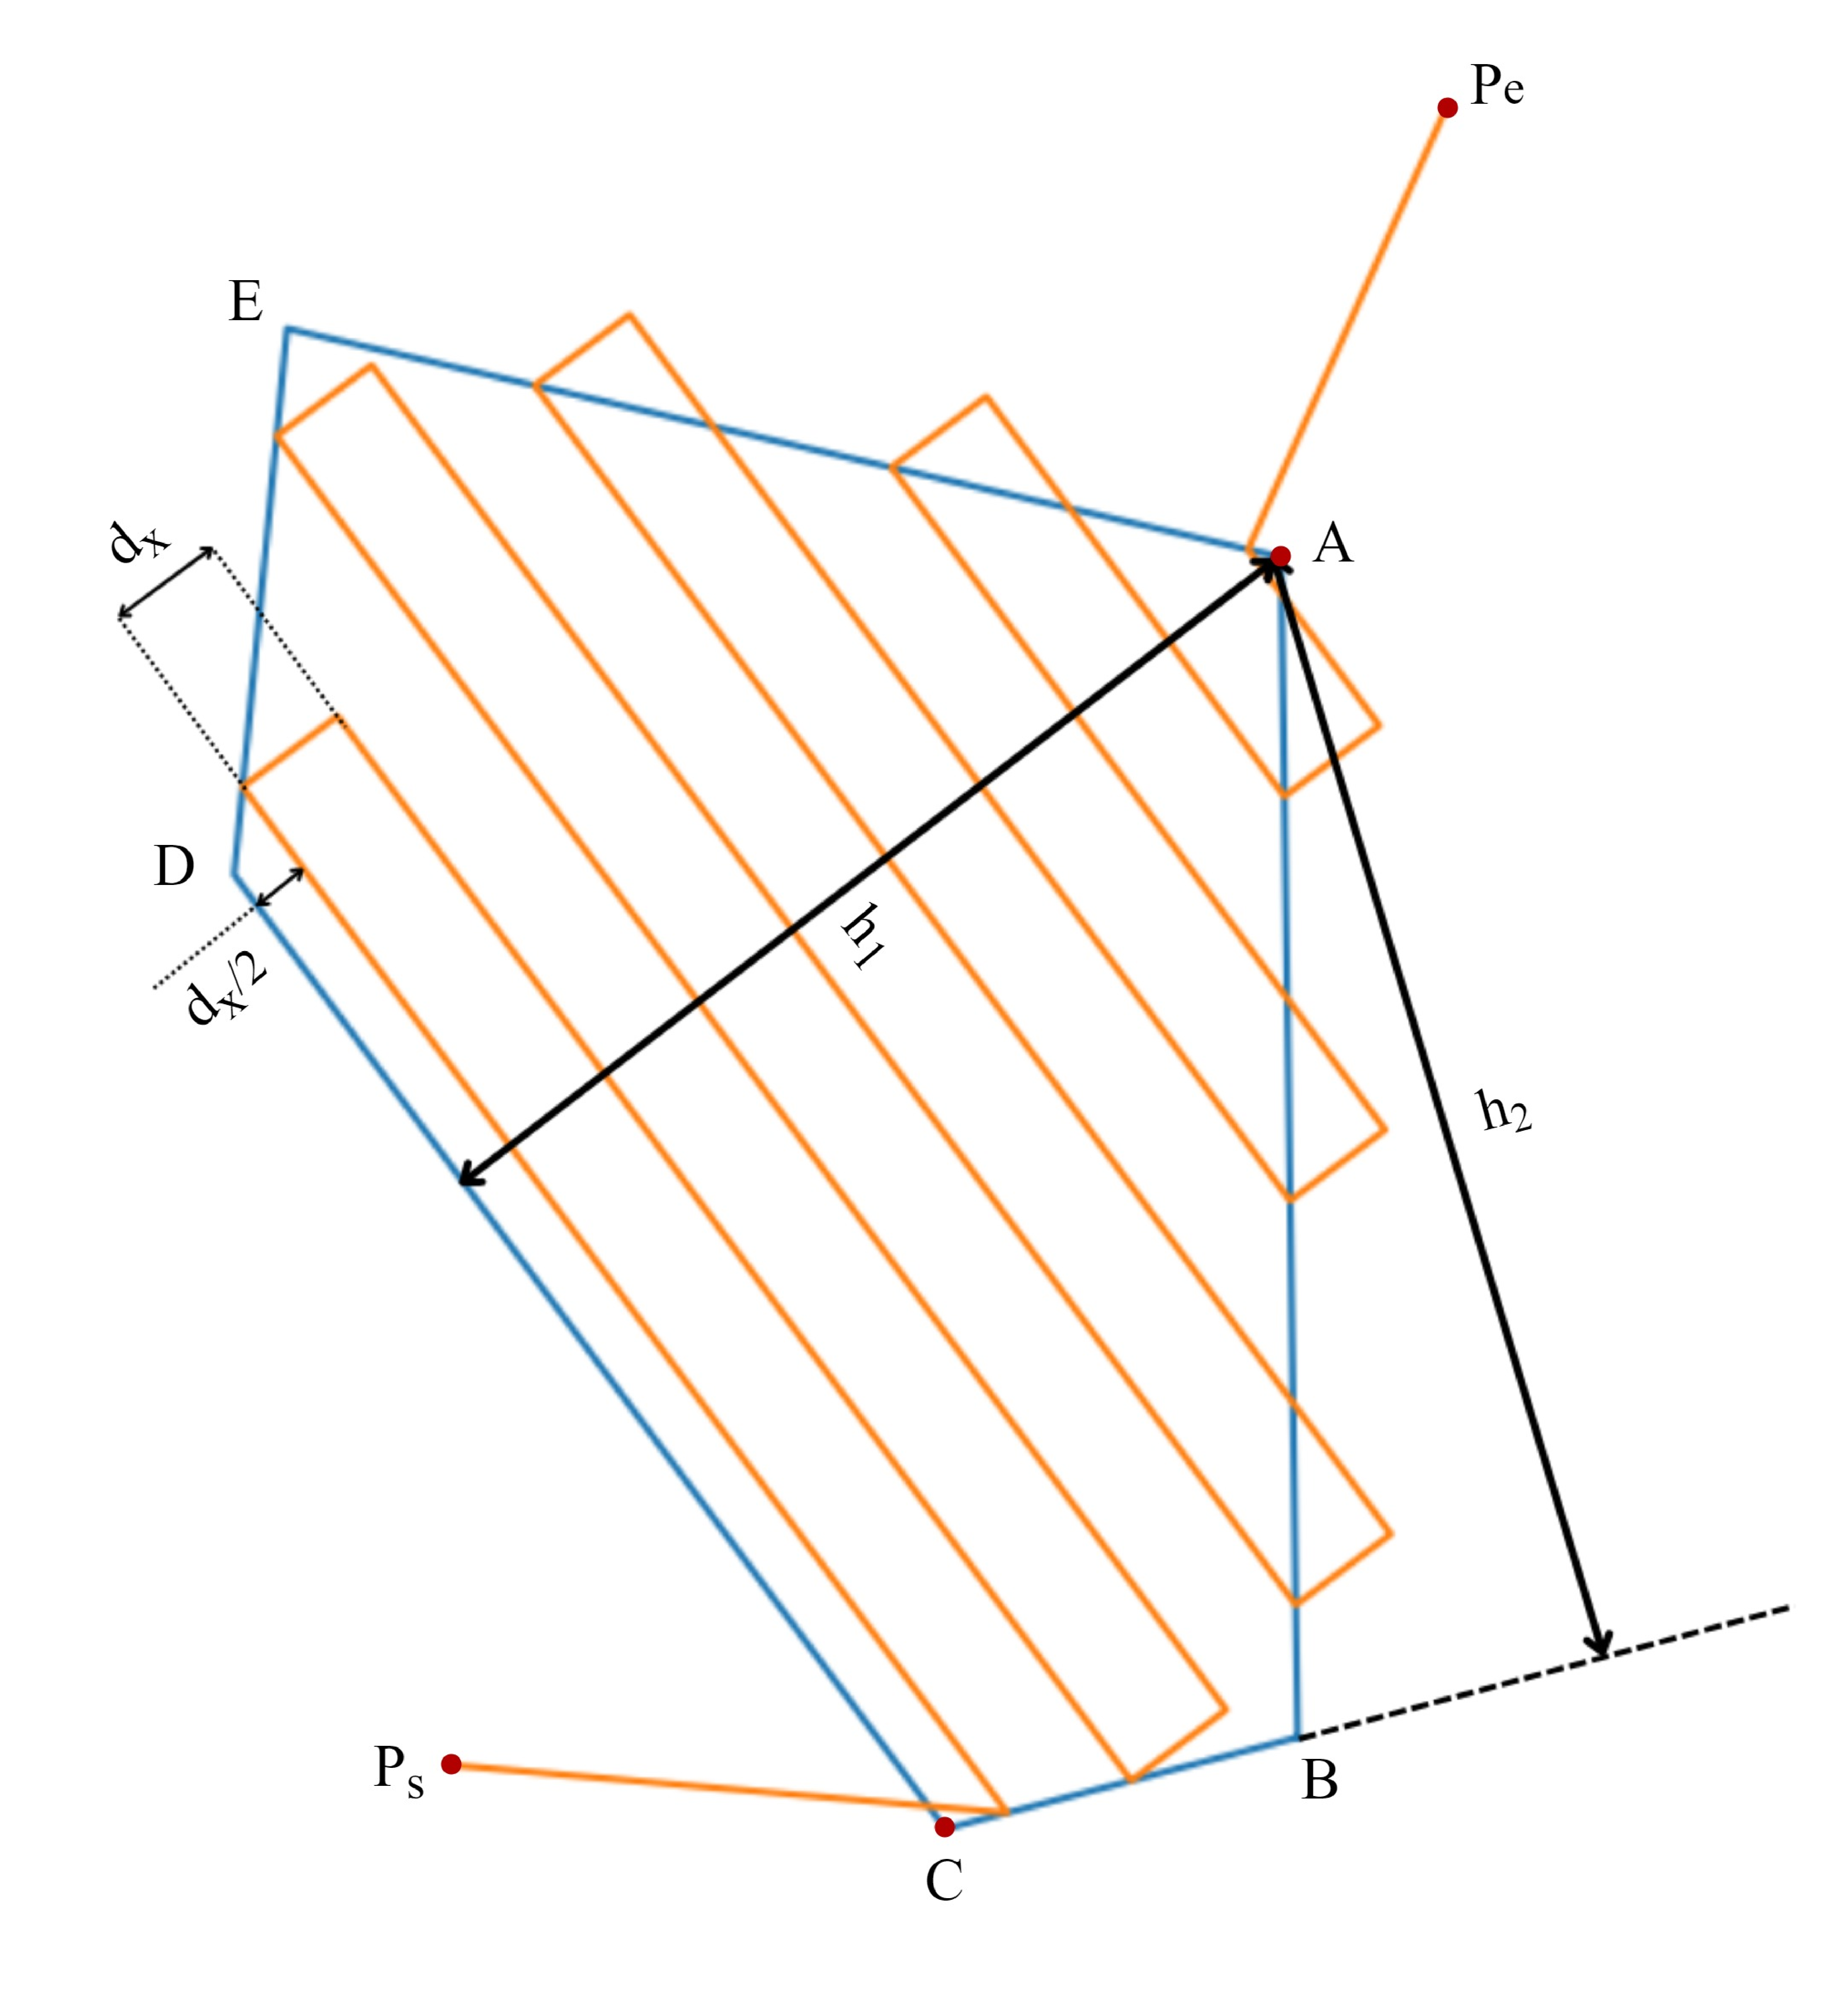
\includegraphics[width=0.5\textwidth]{chapter4/image/sweepline.drawio.pdf}
        \caption{The back-and-forth path is created by RCPP}
        \label{fig:SW1}
    \end{figure}
\section{Đường dẫn bao phủ tối ưu}
\label{subsec:Oppath}
Đường đi của robot quét qua khu vực khảo sát được gọi là đường bao phủ. Nó cần được thiết kế để tối đa hóa vùng phủ sóng và giảm thiểu thời gian bay. Trong điều khiển đội hình, không có sự phân tách khu vực khảo sát nào là cách tiếp cận thích hợp để giải quyết vấn đề này \cite{cabreira2019survey}. Bằng cách đi theo đường gấp khúc \cite{maza2007multiple} cho phép tạo ra các đường quét song song trong khu vực khảo sát. Vì vậy, để thỏa mãn các yêu cầu đã nêu, các đường quét cần đáp ứng các điều kiện sau: quét toàn bộ khu vực khảo sát; giảm thiểu sự chồng chéo giữa vùng phủ sóng của các đường quét; và tối ưu hóa số lượt của bầy Robot.\\

Trong báo cáo này, các đường tới lui(back and forth path) của đỉnh cạnh tối ưu trong khu vực khảo sát bằng cách sử dụng công cụ lập kế hoạch đường dẫn calipers xoay (RCPP) được đề xuất trong \cite{vasquez2020coverage}, và từ đó làm nó trơn tru hơn với nội suy spline khối.
